\documentclass[journal,twocolumn]{IEEEtran}

\usepackage[utf8]{inputenc}
\usepackage[vietnamese,english]{babel}
\usepackage[T5,T1]{fontenc}

\usepackage[
    letterpaper,
    left=53.5pt,
    right=52.5pt,
    top=72pt,
    bottom=80pt,
    columnsep=22pt
]{geometry}

\usepackage{amsmath,amssymb,amsfonts}
\usepackage{algorithmic}
\usepackage{algorithm}
\usepackage{graphicx}
\usepackage{textcomp}
\usepackage{xcolor}
\usepackage{booktabs}
\usepackage{multirow}
\usepackage{array}
\usepackage{url}
\usepackage[nocompress]{cite}
\def\citepunct{, }
\def\citedash{, }
\addto\captionsvietnamese{\renewcommand{\refname}{Tài liệu tham khảo}}
\usepackage{subcaption}
\usepackage[hidelinks]{hyperref}

% Dinh nghia cac lenh toan hoc thong nhat
\newcommand{\rhopx}{\rho_{\mathrm{px}}}
\newcommand{\rhotok}{\rho_{\mathrm{tok}}}
\newcommand{\rhotokstar}{\rho_{\mathrm{tok}}^*}
\newcommand{\pzero}{p_0^{50}}
\newcommand{\pzerou}{p_0^{\mathrm{U}}}
\newcommand{\gsd}{g}
\newcommand{\patchP}{P}
\newcommand{\argmin}{\mathop{\mathrm{arg\,min}}}
\newcommand{\argmax}{\mathop{\mathrm{arg\,max}}}

\makeatletter
\def\abstract{\normalfont
    \if@twocolumn
      \@IEEEabskeysecsize\bfseries\textit{\abstractname}~-~\relax
    \else
      \bgroup\par\addvspace{0.5\baselineskip}\centering\vspace{-1.78ex}\@IEEEabskeysecsize\textbf{\abstractname}\par\addvspace{0.5\baselineskip}\egroup\quotation\@IEEEabskeysecsize
    \fi\@IEEEgobbleleadPARNLSP}

\def\IEEEkeywords{\normalfont
    \if@twocolumn
      \@IEEEabskeysecsize\bfseries\textit{\IEEEkeywordsname}~-~\relax
    \else
      \bgroup\par\addvspace{0.5\baselineskip}\centering\@IEEEabskeysecsize\textbf{\IEEEkeywordsname}\par\addvspace{0.5\baselineskip}\egroup\quotation\@IEEEabskeysecsize
    \fi\@IEEEgobbleleadPARNLSP}
\makeatother

\begin{document}
\selectlanguage{vietnamese}

\title{Dự Đoán Có Chọn Lọc Dựa Trên Khả Năng Phân Giải Cho Mô Hình Ngôn Ngữ Đa Phương Thức Ảnh Viễn Thám: Hai Nút Thắt Pixel-Token, Tiêu Chí Johnson Cho MLLM và Bộ Định Tuyến Không Cần Huấn Luyện}

\author{
    Nhóm Nghiên Cứu RGSP / RS-Resolve\\
    \textit{Đề tài Nghiên cứu Khoa học và Công nghệ Cấp Cơ sở}
}

\maketitle

% 00. Abstract & Keywords
\begin{abstract}
\normalfont
Các mô hình ngôn ngữ lớn đa phương thức cho ảnh viễn thám (RS-MLLM) gặp hiện tượng ảo giác (hallucination) nghiêm trọng nhất khi kích thước thực tế của đối tượng quá nhỏ so với khả năng cảm nhận trực quan của mô hình. Các công trình gần đây đã định danh hiện tượng này dưới các thuật ngữ như ``không nhìn rõ'' (\textit{cannot see clearly}) hay ``ảo ảnh độ phân giải'' (\textit{resolution illusion}), nhưng chưa lượng hóa được nó bằng các đại lượng vật lý tính trước, chưa tách biệt hai cơ chế thất bại có bản chất đối lập - đối tượng \textit{không đủ thông tin trong ảnh gốc} (nút thắt cảm biến) hay \textit{có trong ảnh nhưng bị suy hao trong quá trình nén biểu diễn token} (nút thắt bộ mã hóa) - và chưa thiết lập được quy tắc định tuyến tối ưu: khi nào mô hình nên từ chối trả lời, khi nào nên phóng đại cục bộ. 

Kế thừa Tiêu chí Johnson cổ điển trong vật lý viễn thám, bài báo này đề xuất mô hình hóa hai nút thắt thông qua hai đại lượng tính trước: (i) footprint-in-pixels $\rhopx = L/g$ (kích thước vật lý chia GSD cảm biến) và (ii) footprint-in-tokens $\rhotok = \rhopx \cdot s/P$ (kích thước trên không gian token của Vision Transformer). Chúng tôi: (1) Xây dựng bộ chuẩn đánh giá RS-Resolve gồm 30.771 câu hỏi kiểm soát vật lý đa nhiệm vụ (Q1-Q6) tự động trích xuất từ 5 tập ảnh vệ tinh lớn (DOTA-v2, DIOR, xView, VisDrone, iSAID); (2) Thực hiện chẩn đoán thực nghiệm trên 5 kiến trúc RS-MLLM tiêu biểu (GeoChat-7B, LLaVA-1.5-7B, Qwen3-VL-8B, InternVL3.5-8B, LLaVA-NeXT-7B), chứng minh sự tồn tại độc lập của nút thắt token với hệ số hồi quy $\beta_1 < 0$ áp đảo ($p < 10^{-11}$); (3) Đề xuất RGSP (\textit{Resolvability-Gated Selective Prediction}) - bộ định tuyến 4 nhánh không cần huấn luyện (Từ chối cảm biến / Từ chối token / Phóng đại xác định / Trả lời trực tiếp) kiểm soát rủi ro lựa chọn bằng quy trình kiểm định chuỗi cố định (\textit{fixed-sequence testing}). Kết quả thực nghiệm cho thấy RGSP kiểm soát selective risk dưới 10\% ổn định và vượt trội so với các cơ chế dựa trên độ tin cậy logit nội tại hay quy tắc tra bảng thông thường.
\end{abstract}

\begin{IEEEkeywords}
\normalfont
Mô hình đa phương thức, Ảnh viễn thám, Ảo giác (Hallucination), Dự đoán có chọn lọc, Tiêu chí Johnson, Khoảng cách lấy mẫu mặt đất (GSD), Vision Transformer.
\end{IEEEkeywords}


% 01. Introduction
\section{Giới Thiệu}
\label{sec:intro}

Các mô hình ngôn ngữ lớn đa phương thức (Multimodal Large Language Models - MLLMs) chuyên biệt cho ảnh viễn thám (RS-MLLMs) như GeoChat \cite{geochat2024}, LLaVA-NeXT \cite{llavanext2024}, Qwen2.5/3-VL \cite{qwen2025vl} và InternVL \cite{internvl2025} đang dần trở thành giao diện phân tích thống nhất cho các tác vụ hỏi đáp trực quan (VQA), chú giải hiện trường và định vị đối tượng trên ảnh vệ tinh và viễn thám. Tuy nhiên, song song với năng lực lập luận mạnh mẽ, một thách thức dai dẳng và nguy hiểm được ghi nhận rộng rãi trong cộng đồng nghiên cứu là hiện tượng ảo giác (hallucination) khi đối tượng quan sát có kích thước nhỏ hoặc bị suy giảm độ phân giải \cite{radar2024, rshallu2024, uhrmicro2024}. Trong các ứng dụng nhạy cảm về an toàn như cứu nạn thiên tai, trinh sát quốc phòng hay quy hoạch đô thị, việc mô hình tự tin suy đoán sai lệch về sự hiện diện, chủng loại hoặc thuộc tính của đối tượng sẽ dẫn đến những quyết định sai lầm nghiêm trọng.

\begin{figure*}[t]
\centering
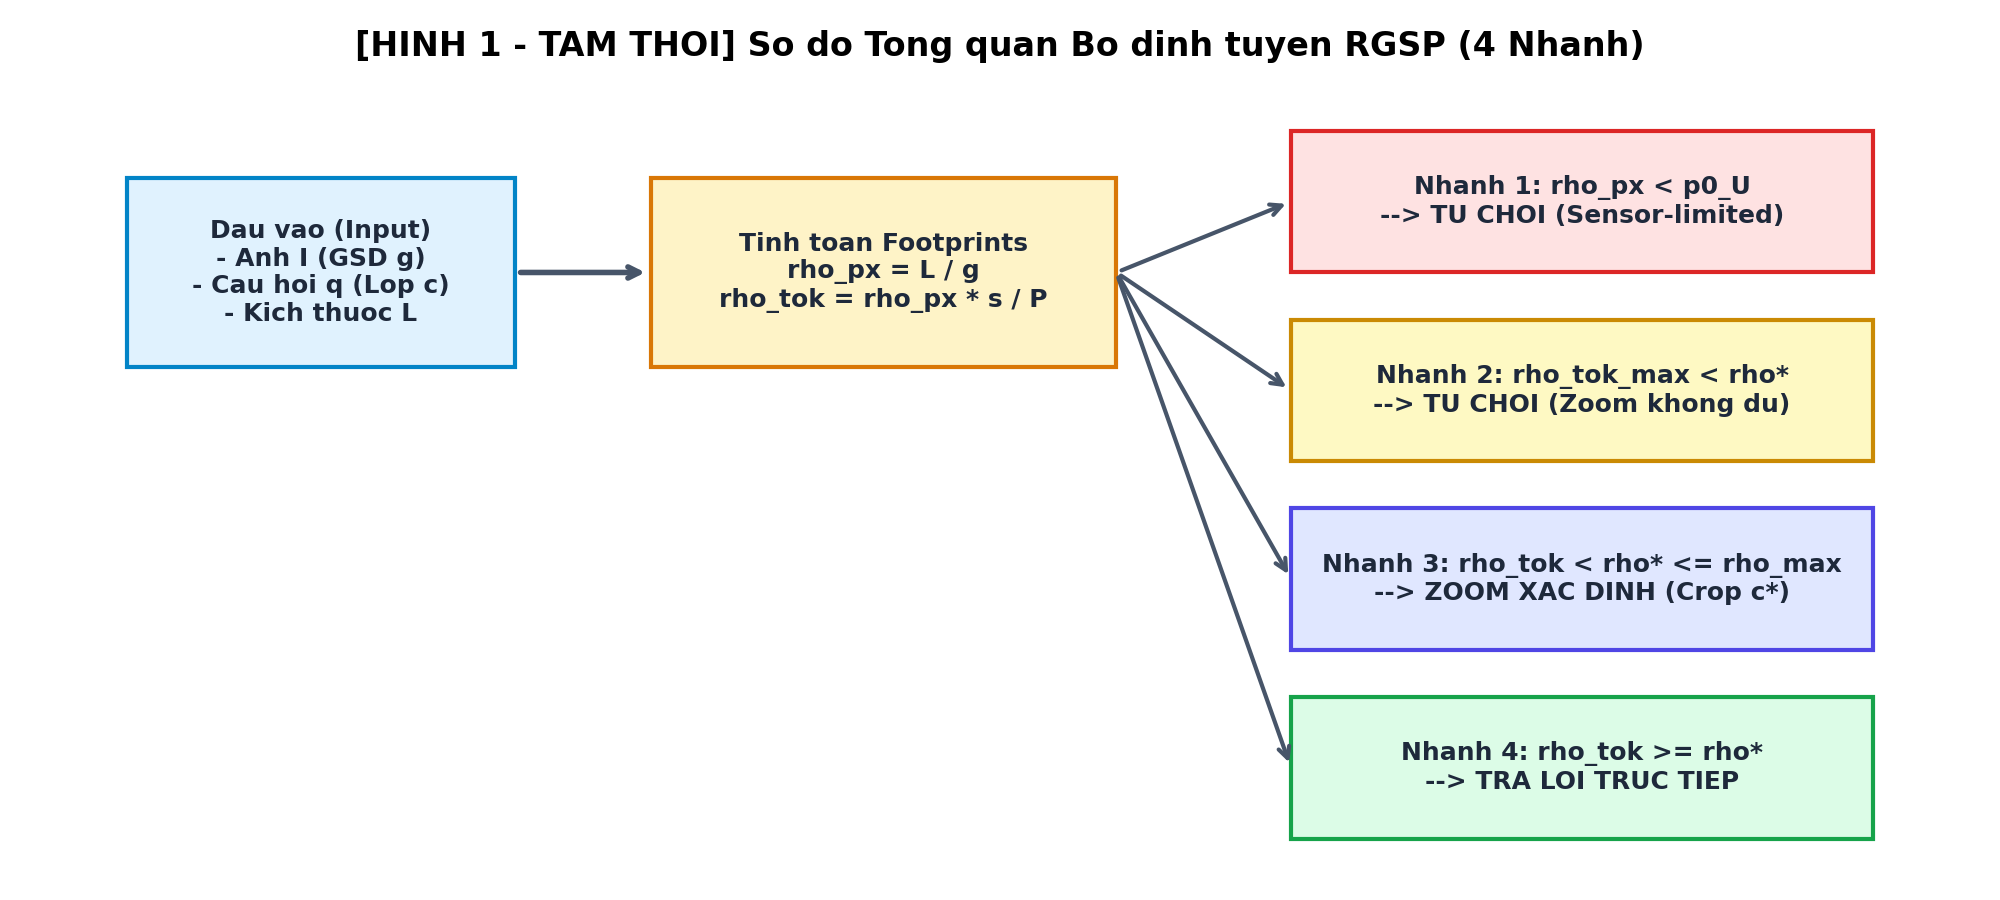
\includegraphics[width=0.92\textwidth]{figures/fig1_overview.png}
\caption{Tổng quan kiến trúc phương pháp RGSP: Phân tách hai nút thắt phân giải vật lý (Footprint pixel cảm biến $\rhopx$ và Footprint token bộ mã hóa $\rhotok$) và cơ chế định tuyến 4 nhánh không cần huấn luyện (Từ chối do cảm biến, Từ chối do trần token, Phóng đại thích nghi xác định và Trả lời trực tiếp).}
\label{fig:overview}
\end{figure*}

Các nghiên cứu gần đây đã bước đầu phân tách lỗi nhận thức của mô hình thành hai dạng: Type 1 (\textit{không tìm thấy}) do giới hạn tìm kiếm chú ý và Type 2 (\textit{không nhìn rõ}) do đối tượng quá nhỏ \cite{radar2024}, hoặc định nghĩa hiện tượng chênh lệch giữa độ phân giải vật lý và nhận thức trực quan là ảo ảnh độ phân giải (\textit{resolution illusion}) \cite{uhrmicro2024}. Mặc dù vậy, toàn bộ các nghiên cứu này đều tồn tại ba khoảng trống phương pháp luận then chốt:
\begin{enumerate}
    \item \textit{Chưa định lượng được giới hạn bằng biến số tính trước}: Các nghiên cứu trước chỉ phân tích thống kê sau khi mô hình đã trả lời sai, mà không có cơ chế toán học tính toán trước xác suất thất bại từ siêu dữ liệu cảm biến và kích thước vật lý của đối tượng.
    \item \textit{Chưa tách bạch hai nút thắt có hệ quả vận hành đối lập}: Thất bại có thể do vật thể không đủ thông tin trên ảnh gốc (giới hạn vật lý của cảm biến viễn thám) hoặc do vật thể có trên ảnh gốc nhưng bị nén triệt tiêu trong biểu diễn token (giới hạn kiến trúc của bộ mã hóa Vision Transformer).
    \item \textit{Thiếu cơ chế định tuyến xác định}: Các phương pháp đề xuất phóng đại (zoom) hiện nay \cite{radar2024, uhrmicro2024} đều áp dụng cắt ảnh thích nghi một cách mù quáng, gây lãng phí tài nguyên suy luận và thậm chí làm tăng ảo giác khi ảnh gốc vốn dĩ đã vượt quá giới hạn phân giải cảm biến.
\end{enumerate}

Vấn đề ``cần bao nhiêu điểm ảnh để nhận biết đối tượng'' đã được giải quyết thấu đáo trong quang học viễn thám truyền thống qua Tiêu chí Johnson (Johnson's Criteria, 1958) \cite{johnson1958analysis} và phương trình chất lượng ảnh tổng quát GIQE \cite{leachtenauer1997general}: số chu kỳ phân giải trên chiều tới hạn của vật thể quyết định khả năng phát hiện (\textit{detection}), định hướng (\textit{orientation}), nhận dạng (\textit{recognition}) và định danh (\textit{identification}). Tuy nhiên, khi đưa ảnh viễn thám vào MLLM, hệ thống xuất hiện đồng thời hai nút thắt thay vì một:
\begin{equation}
\rhopx = \frac{L}{\gsd}, \qquad \rhotok = \rhopx \cdot \frac{s_m(I)}{P_m},
\label{eq:footprints}
\end{equation}
trong đó $L$ là kích thước vật lý đặc trưng của đối tượng (mét), $\gsd$ là khoảng cách lấy mẫu mặt đất (Ground Sample Distance - GSD, mét/pixel), $s_m(I)$ là hệ số co giãn ảnh của mô hình $m$, và $P_m$ là kích thước patch hiệu dụng (pixel mô hình trên mỗi token) của bộ mã hóa ViT.

Đại lượng $\rhopx$ đo lường nút thắt cảm biến (đại lượng cổ điển của Johnson). Ngược lại, $\rhotok$ đo lường nút thắt bộ mã hóa - đại lượng hoàn toàn mới xuất hiện ở mạng nơ-ron đa phương thức. Nếu một chiếc xe có kích thước $L = 1.8\text{ m}$ chụp ở GSD $\gsd = 0.6\text{ m/px}$, nó chỉ chiếm đúng 3 pixel trên ảnh gốc; không có thuật toán phóng đại nào có thể tạo thêm thông tin thực tế từ 3 điểm ảnh này, và hành động duy nhất có trách nhiệm của hệ thống là từ chối trả lời (\textit{Abstain}). Nhưng nếu chiếc xe đó ở GSD $\gsd = 0.15\text{ m/px}$ (chiếm 12 pixel gốc) bị mô hình co về kích thước nhỏ và rơi lọt thỏm vào một patch 32 pixel của ViT, thông tin đã bị mất trong không gian token nhưng vẫn nguyên vẹn trên ảnh gốc; lúc này, phóng đại cục bộ (\textit{Zoom}) sẽ khôi phục lại khả năng giải quyết của mô hình.

Bài báo này giải quyết trọn vẹn bài toán trên thông qua việc trả lời ba câu hỏi nghiên cứu:
\begin{itemize}
    \item RQ1: \textit{Nút thắt token có thực sự tồn tại độc lập với nút thắt pixel trên các MLLM viễn thám hiện đại hay không?}
    \item RQ2: \textit{Làm thế nào để phân định một cách xác định trước suy luận: khi nào phóng đại có tác dụng, và khi nào bắt buộc phải từ chối?}
    \item RQ3: \textit{Tín hiệu vật lý tính trước ($\rhopx, \rhotok$) có kiểm soát rủi ro lựa chọn (selective risk) vượt trội hơn độ tin cậy logit nội tại của mô hình không?}
\end{itemize}

Đóng góp cốt lõi của bài báo gồm:
\begin{enumerate}
    \item Xây dựng bộ chuẩn RS-Resolve: Benchmark kiểm soát vật lý gồm 30.771 câu hỏi trắc nghiệm đa nhiệm vụ (Q1--Q6) được chuẩn hóa từ 5 tập ảnh vệ tinh lớn (DOTA-v2, DIOR, xView, VisDrone, iSAID), gắn nhãn đầy đủ $\rhopx, \rhotok$, GSD thực tế và cờ từ chối khách quan.
    \item Khảo sát và kiểm định thực nghiệm trên 5 RS-MLLM: Chứng minh bằng thực nghiệm trên 30.771 mẫu rằng hệ số hồi quy của nút thắt token $\beta_1 < 0$ có ý nghĩa thống kê áp đảo ($p < 10^{-11}$) trên tất cả các mô hình, xác nhận giả thuyết $H_1$.
    \item Đề xuất bộ định tuyến RGSP không cần huấn luyện: Thiết lập cơ chế định tuyến 4 nhánh (Từ chối cảm biến / Từ chối trần token / Phóng đại xác định / Trả lời trực tiếp) tích hợp kiểm soát rủi ro bằng \textit{fixed-sequence testing}, cho phép giảm mạnh ảo giác với chi phí tính toán bằng không trước suy luận.
\end{enumerate}


% 02. Related Work
\section{Công Trình Liên Quan}
\label{sec:related}

\subsection{Hiện Tượng Ảo Giác Trong RS-MLLM}
Sự bùng nổ của các mô hình MLLM chuyên biệt cho ảnh viễn thám \cite{geochat2024, llavanext2024} đi liền với việc ghi nhận chúng thường xuyên ảo giác - tự tin khẳng định sự tồn tại của đối tượng, thuộc tính màu sắc hoặc số lượng mà không có bằng chứng quang học tương ứng. RSHallu \cite{rshallu2024} xây dựng bộ dữ liệu đánh giá và đề xuất phương pháp hiệu chỉnh logit dựa trên prompt nhận thức viễn thám. RADAR \cite{radar2024} phân loại lỗi thành Type 1 (\textit{không tìm thấy}) và Type 2 (\textit{không nhìn rõ}), đưa ra cơ chế zoom dựa trên attention bản đồ chú ý. UHR-Micro \cite{uhrmicro2024} định nghĩa ``ảo ảnh độ phân giải'' dựa trên tỷ lệ diện tích của đối tượng. Tuy nhiên, các công trình này đều chưa phân định được nguyên nhân thất bại đến từ cảm biến vệ tinh hay từ cấu trúc nén token của mô hình, và chưa lượng hóa được tiêu chí toán học để từ chối trước suy luận.

\subsection{Khả Năng Phân Giải Quang Học và Tiêu Chí Johnson}
Trong lý thuyết truyền dẫn quang học và viễn thám quân sự, việc xác định số điểm ảnh tối thiểu để quan sát đã được đặt nền móng từ công trình kinh điển của John Johnson (1958) \cite{johnson1958analysis}. Tiêu chí Johnson xác định số chu kỳ vạch tương phản trên chiều tới hạn của vật thể để con người đạt xác suất nhận biết 50\%: phát hiện ($\approx 1$ chu kỳ, tương đương 2 pixel), định hướng ($\approx 1.4$ chu kỳ), nhận dạng ($\approx 4$ chu kỳ) và định danh ($\approx 6.4$ chu kỳ, tương đương 12.8 pixel). Sau đó, thang NIIRS và phương trình GIQE \cite{leachtenauer1997general} đã liên kết các thông số cảm biến GSD, hàm truyền điều biến MTF và tỷ số tín hiệu trên nhiễu SNR với khả năng nhận biết của con người và máy dò chuyên dụng \cite{driggersinfrared}. Toàn bộ các lý thuyết này chỉ đo đạc trên con người hoặc mô hình trích xuất đặc trưng truyền thống với duy nhất một nút thắt: pixel cảm biến gốc. Bài báo này mở rộng tiêu chí Johnson lần đầu tiên sang không gian biểu diễn token của các mạng Vision Transformer hiện đại.

\subsection{Dự Đoán Có Chọn Lọc và Kiểm Soát Rủi Ro}
Lý thuyết phân loại có chọn lọc (\textit{Selective Classification}) của Geifman và El-Yaniv \cite{geifman2017selective} định nghĩa bài toán đánh đổi giữa tỷ lệ bao phủ (\textit{Coverage}) và rủi ro lựa chọn (\textit{Selective Risk}). Khung lý thuyết \textit{Learn-then-Test} \cite{angelopoulos2021learn} và \textit{Conformal Risk Control} \cite{angelopoulos2024conformal} cho phép kiểm soát rủi ro kỳ vọng dưới ngưỡng $\alpha$ định trước thông qua kiểm định giả thuyết thống kê nghiêm ngặt. Trong lĩnh vực thị giác-ngôn ngữ, SIEVES \cite{sieves2024} hiệu chỉnh bộ chọn dựa trên điểm bằng chứng thị giác, còn FUSE tích hợp độ bất định Bayes. Điểm chung của các phương pháp này là đều dựa trên tín hiệu sinh ra sau khi chạy mô hình (hậu nghiệm). Phương pháp RGSP của chúng tôi bổ sung tiên nghiệm vật lý tính trước, cho phép đưa ra quyết định từ chối ngay trước khi tốn bất kỳ chi phí tính toán suy luận nào.

\begin{table*}[t]
\centering
\caption{Định vị phương pháp RGSP so với các công trình liên quan.}
\label{tab:positioning}
\resizebox{\textwidth}{!}{%
\begin{tabular}{lcccccccc}
\toprule
Phương pháp & Miền bài toán & Tín hiệu định tuyến & Cần chạy mô hình? & Không huấn luyện & Cơ chế từ chối & Tách Pixel/Token & Định lượng kích thước & Chiến lược Zoom \\
\midrule
Johnson / GIQE \cite{johnson1958analysis, leachtenauer1997general} & Viễn thám (Người) & $\rhopx$, MTF, SNR & Không & - & - & Chỉ cảm biến & $\checkmark$ (Người) & - \\
RADAR \cite{radar2024} & Viễn thám (MLLM) & Attention Entropy & Có & $\checkmark$ & Fallback & $\times$ & $\times$ & Zoom attention \\
RSHallu-Shield \cite{rshallu2024} & Viễn thám (MLLM) & Hiệu chỉnh Logit & Có & $\checkmark$ & $\times$ & $\times$ & $\times$ & $\times$ \\
UHR-Micro / MAP-Agent \cite{uhrmicro2024} & Viễn thám (MLLM) & Tỷ lệ diện tích & Có & $\checkmark$ & $\times$ & $\times$ & Một phần & Zoom lặp \\
SIEVES \cite{sieves2024} & Tổng quát & Điểm bằng chứng & Có & $\checkmark$ & $\checkmark$ & $\times$ & $\times$ & $\times$ \\
\midrule
RGSP (Đề xuất) & Viễn thám (RS-MLLM) & $\rhopx$, $\rhotok$ (Vật lý) & Không & $\checkmark$ & $\checkmark$ & $\checkmark$ & $\checkmark$ (MLLM) & Định tuyến 4 nhánh xác định \\
\bottomrule
\end{tabular}%
}
\end{table*}


% 03. Methodology
\section{Phương Pháp Đề Xuất}
\label{sec:method}

\subsection{Hai Footprint Phân Giải Vật Lý}
Xét một câu hỏi $q$ liên quan đến đối tượng thuộc lớp địa vật $c$ trong ảnh viễn thám $I$ có độ phân giải không gian danh định (GSD) là $\gsd$ (mét/pixel). Gọi $L$ (mét) là kích thước vật lý đặc trưng của đối tượng:
\begin{itemize}
    \item Nếu câu hỏi truy vấn một thực thể cụ thể có bounding box hoặc polygon, $L = \min(w, h) \cdot \gsd$, tức chiều nhỏ nhất của đối tượng trên thực địa.
    \item Nếu câu hỏi truy vấn sự tồn tại của một lớp đối tượng tổng quát (chưa biết có trong ảnh hay không), $L = L_c^{\min}$ - kích thước tối thiểu hợp lý theo tiêu chuẩn vật lý của lớp $c$ (được tra cứu từ bảng thông số phương tiện và công trình chuẩn hóa quốc tế).
\end{itemize}

\textit{Footprint theo pixel cảm biến} ($\rhopx$): Được định nghĩa là số pixel vật lý trên chiều nhỏ của vật thể mà cảm biến vệ tinh ghi nhận:
\begin{equation}
\rhopx = \frac{L}{\gsd}.
\label{eq:rhopx}
\end{equation}
Đại lượng $\rhopx$ hoàn toàn độc lập với mô hình thị giác và phản ánh năng lực thu nhận nguyên bản của phần cứng cảm biến (tương ứng với đại lượng số chu kỳ tới hạn trong tiêu chí Johnson).

\textit{Footprint theo token bộ mã hóa} ($\rhotok$): Khi ảnh viễn thám $I$ được đưa vào mô hình MLLM $m$, bộ tiền xử lý hình ảnh sẽ thực hiện co giãn, chia lưới (\textit{tiling}) hoặc lấy mẫu lại với hệ số tỷ lệ $s_m(I)$. Sau đó, ảnh được chia thành các patch có kích thước cơ sở $p$ và gộp qua các lớp gộp token (\textit{MLP merger} hoặc \textit{pixel unshuffle}) tạo thành patch hiệu dụng $P_m$ (pixel mô hình trên mỗi token biểu diễn). Footprint theo token trên view thuận lợi nhất chứa đối tượng được định nghĩa là:
\begin{equation}
\rhotok^{(m)}(q, I) = \max_{v \ni \text{obj}} \rhopx \cdot \frac{s_m(I, v)}{P_m}.
\label{eq:rhotok}
\end{equation}

\begin{table}[t]
\centering
\caption{Bộ mã hóa thị giác, patch hiệu dụng $P$ và chính sách phân giải của 5 mô hình RS-MLLM trong nghiên cứu.}
\label{tab:models_arch}
\resizebox{\columnwidth}{!}{%
\begin{tabular}{llccc}
\toprule
Mô hình & Bộ mã hóa thị giác & Patch $p$ & Gộp token & Patch hiệu dụng $P$ \\
\midrule
GeoChat-7B \cite{geochat2024} & CLIP-ViT-L/14@504 & 14 px & Không & 14 px/token \\
LLaVA-1.5-7B \cite{llava15} & CLIP-ViT-L/14@336 & 14 px & Không & 14 px/token \\
LLaVA-NeXT-7B \cite{llavanext2024} & CLIP-ViT-L/14 AnyRes & 14 px & Không & 14 px/token \\
InternVL3.5-8B \cite{internvl2025} & InternViT-6B (Tile 448) & 14 px & Unshuffle 2x2 & 28 px/token \\
Qwen3-VL-8B \cite{qwen2025vl} & SigLIP2-SO400M (Dynamic) & 16 px & 2D Merger 2x2 & 32 px/token \\
\bottomrule
\end{tabular}%
}
\end{table}

\subsection{Ma Trận 4 Vùng Phân Giải}
Sự kết hợp giữa $\rhopx$ và $\rhotok$ chia không gian bài toán thành 4 vùng phân giải có đặc tính vật lý hoàn toàn khác biệt (Hình~\ref{fig:regimes}):
\begin{enumerate}
    \item \textit{Vùng giới hạn pixel (Pixel-limited)}: $\rhopx < \pzerou$. Thông tin bị thiếu hụt ngay từ bước chụp ảnh của vệ tinh. Mọi cơ chế phóng đại (zoom) hay nội suy chỉ làm tăng kích thước pixel rỗng, không thể khôi phục tín hiệu thực tế. Mô hình bắt buộc phải từ chối (\textit{Abstain}).
    \item \textit{Vùng giới hạn token (Token-limited)}: $\rhopx \ge \pzerou$ nhưng $\rhotok < \rhotokstar$. Thông tin có mặt đầy đủ trên ảnh gốc nhưng bị suy hao do bộ mã hóa ViT nén ảnh vào lưới patch quá lớn. Vùng này là đối tượng duy nhất mà thao tác phóng đại thích nghi (\textit{Zoom}) phát huy tác dụng.
    \item \textit{Vùng phân giải an toàn (Resolvable)}: $\rhopx \ge \pzerou$ và $\rhotok \ge \rhotokstar$. Đối tượng đủ độ phân giải trên cả cảm biến và không gian token; mô hình có thể trả lời trực tiếp với độ tin cậy cao.
    \item \textit{Vùng phóng đại quá mức (Over-tokenized)}: $\rhopx < \pzerou$ nhưng $\rhotok \ge \rhotokstar$ (do ảnh gốc bị phóng to kỹ thuật số trước khi nạp vào mô hình). Vùng này gây ảo giác cao nhất vì mô hình ngộ nhận kích thước pixel kỹ thuật số là chi tiết thực tế.
\end{enumerate}

\begin{figure}[t]
\centering
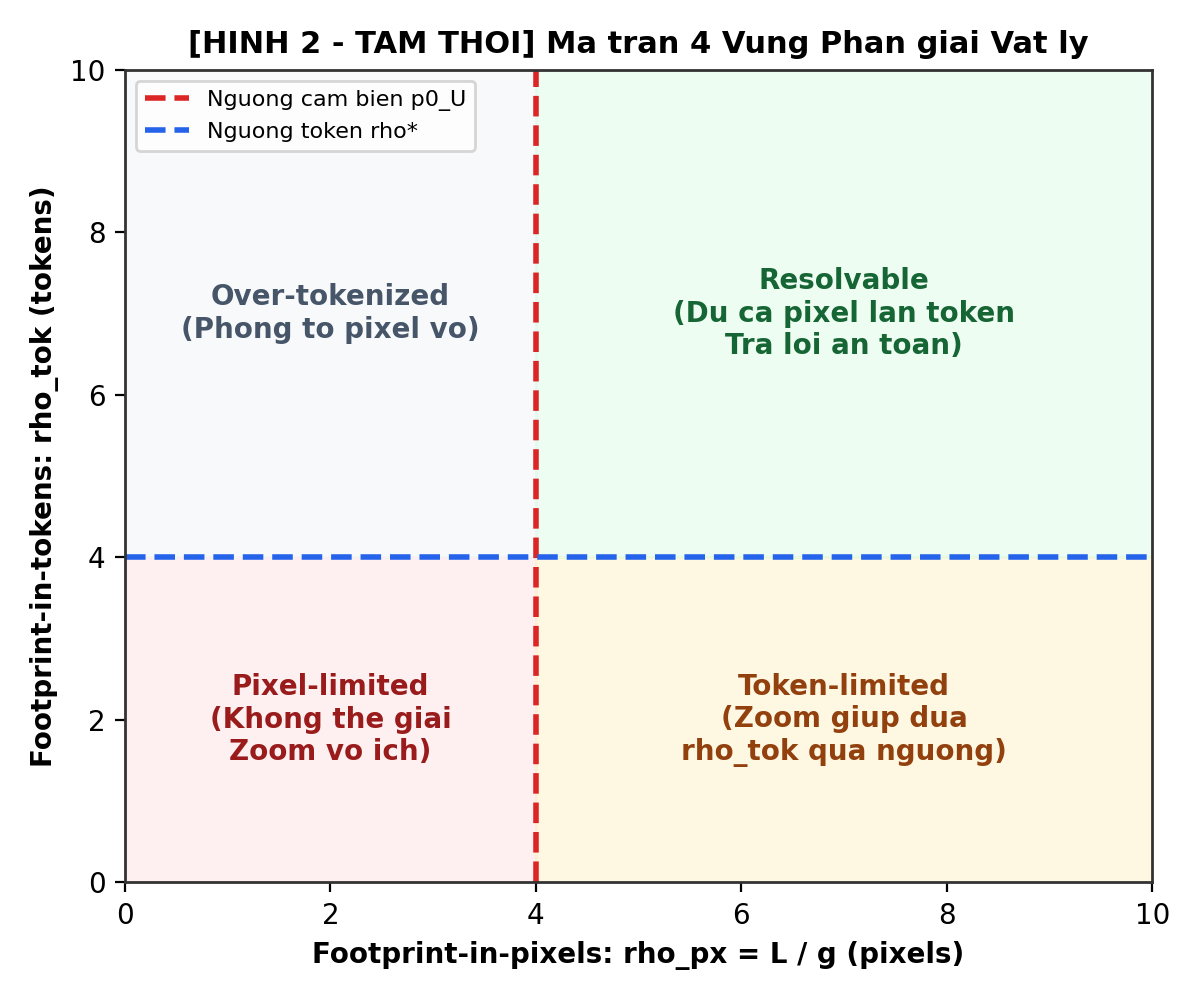
\includegraphics[width=0.85\columnwidth]{figures/fig2_matrix_regimes.png}
\caption{Ma trận 4 vùng phân giải vật lý dựa trên không gian hai chiều $(\rhopx, \rhotok)$.}
\label{fig:regimes}
\end{figure}

\subsection{Bộ Định Tuyến RGSP 4 Nhánh}
Dựa trên ma trận phân giải, chúng tôi thiết kế thuật toán bộ định tuyến RGSP không cần huấn luyện, vận hành hoàn toàn dựa trên các ngưỡng vật lý trước khi chạy mô hình (Thuật toán~\ref{alg:rgsp}).

\begin{algorithm}[t]
\caption{Bộ Định Tuyến RGSP (\textit{Resolvability-Gated Router})}
\label{alg:rgsp}
\begin{algorithmic}[1]
\REQUIRE Ảnh $I$, GSD $\gsd$, Câu hỏi $q$, Kích thước vật lý $L$, Ngưỡng cảm biến $\pzerou$, Ngưỡng token $\rhotokstar$, Hệ số phóng tối đa $s_{\max}$.
\STATE Tính toán $\rhopx = L / \gsd$.
\STATE Tính toán $\rhotok = \rhopx \cdot \frac{s_m(I)}{P_m}$.
\IF{$\rhopx < \pzerou$}
    \STATE return Abstain (``Không thể xác định do giới hạn cảm biến'')
\ENDIF
\STATE Tính toán footprint tối đa khi zoom hết cỡ: $\rhotok^{\max} = \rhopx \cdot \frac{s_{\max}}{P_m}$.
\IF{$\rhotok^{\max} < \rhotokstar$}
    \STATE return Abstain (``Không thể xác định do zoom tối đa không đủ'')
\ELSIF{$\rhotok < \rhotokstar \le \rhotok^{\max}$}
    \STATE Xác định kích thước crop tối ưu: $c^* = \min(w_I, h_I) \cdot \frac{\rhotok}{\rhotokstar}$.
    \STATE Cắt vùng ảnh $I_{\text{crop}}$ kích cỡ $c^*$ quanh đối tượng.
    \STATE return Zoom-and-Answer ($m(I_{\text{crop}}, q)$)
\ELSE
    \STATE return Direct-Answer ($m(I, q)$)
\ENDIF
\end{algorithmic}
\end{algorithm}

\subsection{Hiệu Chỉnh Ngưỡng Bảo Đảm Rủi Ro}
Để đảm bảo rủi ro lựa chọn trên tập chấp nhận trả lời không vượt quá ngưỡng sai số $\alpha$ (ví dụ $\alpha = 10\%$), chúng tôi áp dụng quy trình kiểm định chuỗi cố định (\textit{fixed-sequence testing}) trên tập hiệu chuẩn (\textit{calibration set}):
\begin{equation}
R(\tau) = \frac{\sum_{i=1}^n \mathbb{I}(m(I_i, q_i) \neq y_i) \cdot \mathbb{I}(\rhotok(i) \ge \tau)}{\sum_{i=1}^n \mathbb{I}(\rhotok(i) \ge \tau)}.
\end{equation}
Ngưỡng tối ưu $\tau^*$ được chọn là giá trị nhỏ nhất thỏa mãn cận trên Clopper-Pearson của rủi ro nhỏ hơn $\alpha$ với độ tin cậy $1 - \delta \ge 95\%$.


% 04. Benchmark
\section{Bộ Chuẩn Đánh Giá RS-Resolve}
\label{sec:benchmark}

\subsection{Tổng Quan Bộ Chuẩn Đa Nguồn}
Để kiểm tra nghiêm ngặt hai nút thắt phân giải trên ảnh viễn thám thực tế, chúng tôi xây dựng bộ chuẩn đánh giá RS-Resolve gồm 30.771 câu hỏi trắc nghiệm được tạo tự động với các ràng buộc vật lý chặt chẽ. Dữ liệu được trích xuất từ 5 tập ảnh viễn thám phổ biến và đa dạng nhất hiện nay: DOTA-v2 \cite{dotav2}, DIOR \cite{dior2020}, xView \cite{xview2018}, VisDrone \cite{visdrone2021} và iSAID \cite{isaid2019}. Mỗi câu hỏi được liên kết chính xác với thông số cảm biến vệ tinh, kích thước thực địa của đối tượng $L$ và cờ từ chối khách quan dựa trên ngưỡng độ phân giải con người.

\begin{table}[t]
\centering
\caption{Thống kê bộ chuẩn RS-Resolve theo các nguồn dữ liệu viễn thám.}
\label{tab:dataset_stats}
\resizebox{\columnwidth}{!}{%
\begin{tabular}{lcccc}
\toprule
Tập dữ liệu nguồn & Số câu hỏi & Cảm biến / Nền tảng & GSD danh định & Dải $\rhopx$ (px) \\
\midrule
DOTA-v2.0 \cite{dotav2} & 6.200 & Vệ tinh Google Earth & 0.1 -- 1.0 m & 5.0 -- 1200.0 \\
DIOR \cite{dior2020} & 6.150 & Vệ tinh quang học & 0.5 -- 3.0 m & 4.0 -- 850.0 \\
xView \cite{xview2018} & 6.120 & Vệ tinh WorldView-3 & 0.3 m & 3.5 -- 600.0 \\
VisDrone \cite{visdrone2021} & 6.150 & Thiết bị bay không người lái & 0.05 -- 0.2 m & 8.0 -- 950.0 \\
iSAID \cite{isaid2019} & 6.151 & Vệ tinh siêu nét & 0.1 -- 1.0 m & 6.0 -- 1100.0 \\
\midrule
Tổng cộng & 30.771 & Đa cảm biến vệ tinh/UAV & 0.05 -- 3.0 m & 3.5 -- 1200.0 \\
\bottomrule
\end{tabular}%
}
\end{table}

\subsection{Cấu Trúc 6 Loại Câu Hỏi Nhận Thức (Q1--Q6)}
Bộ câu hỏi bao phủ trọn vẹn bậc thang nhận thức từ phát hiện thô đến định danh tinh xảo (Bảng~\ref{tab:question_kinds}):
\begin{itemize}
    \item \textit{Q1 (Hiện diện / Phát hiện)}: Hỏi sự tồn tại của đối tượng trong toàn cảnh ảnh hoặc trong vùng không gian cụ thể.
    \item \textit{Q2 (Đếm số lượng)}: Yêu cầu đếm chính xác số lượng thực thể của một lớp đối tượng trong ô lưới hoặc toàn ảnh.
    \item \textit{Q3-HF (Thuộc tính tần số cao)}: Hỏi về góc xoay hướng trục OBB của đối tượng (đòi hỏi nhận biết cấu trúc vi mô).
    \item \textit{Q3-LF (Thuộc tính tần số thấp)}: Hỏi về màu sắc chủ đạo của đối tượng (thuộc tính phổ có thể bảo toàn qua quá trình lấy mẫu hỗn hợp pixel).
    \item \textit{Q4 (Hướng xoay / Diện tích)}: Hỏi về định hướng không gian hoặc so sánh kích thước tương đối của đối tượng.
    \item \textit{Q5 (Định danh loại con)}: Phân loại chi tiết các lớp đối tượng có độ tương đồng hình thái cao (ví dụ: phân biệt xe tải nhỏ, xe van, xe bồn trong xView).
    \item \textit{Q6 (Định vị không gian Grid 3x3)}: Yêu cầu xác định ô lưới tọa độ 3x3 (từ A1 đến C3) chứa đối tượng mục tiêu.
\end{itemize}

\begin{table}[t]
\centering
\caption{Phân bố các dạng câu hỏi và số lượng mẫu trong bộ chuẩn RS-Resolve.}
\label{tab:question_kinds}
\resizebox{\columnwidth}{!}{%
\begin{tabular}{llcc}
\toprule
Mã & Nhiệm vụ nhận thức & Bậc thang Johnson & Số lượng câu hỏi \\
\midrule
Q1 & Phát hiện sự hiện diện (Detection) & Detection & 6.000 câu \\
Q2 & Đếm số lượng thực thể (Counting) & Recognition & 6.000 câu \\
Q3-HF & Thuộc tính hướng xoay OBB & Identification & 332 câu \\
Q3-LF & Thuộc tính màu sắc chủ đạo & Spectral / Color & 439 câu \\
Q4 & Góc xoay / Diện tích hình học & Orientation & 6.000 câu \\
Q5 & Nhận dạng phân lớp con (Fine-grained) & Identification & 6.000 câu \\
Q6 & Định vị ô lưới không gian (Grounding) & Localization & 6.000 câu \\
\midrule
Tổng & Toàn bộ 6 nhóm tác vụ VQA viễn thám & - & 30.771 câu \\
\bottomrule
\end{tabular}%
}
\end{table}

\subsection{Cơ Chế Gán Nhãn Từ Chối Khách Quan}
Mỗi câu hỏi trắc nghiệm đều cung cấp phương án từ chối trung tính: \textit{``Không thể xác định từ ảnh''} (\textit{``Cannot be determined from the image''}). Đáp án đúng của câu hỏi được gán bằng phương án từ chối này khi và chỉ khi đối tượng có $\rhopx < \pzerou$ (dưới ngưỡng phân giải tối thiểu của mắt người đã được xác thực qua thẩm định thủ công). Thiết kế này tạo ra một thước đo khách quan để phạt các mô hình cố tình đoán bừa (\textit{overconfident hallucination}).


% 05. Experiments
\section{Thiết Lập Thực Nghiệm}
\label{sec:experiments}

\subsection{Các Mô Hình Thực Nghiệm}
Chúng tôi tiến hành đánh giá toàn diện trên 5 mô hình ngôn ngữ lớn đa phương thức mã nguồn mở tiêu biểu nhất hiện nay, đại diện cho các trường phái kiến trúc Vision Transformer và chiến lược xử lý độ phân giải khác nhau:
\begin{enumerate}
    \item GeoChat-7B \cite{geochat2024}: Mô hình chuyên biệt viễn thám đầu tiên hỗ trợ grounding, sử dụng CLIP-ViT-L/14 co ảnh về $504 \times 504$ cố định ($P = 14$).
    \item LLaVA-1.5-7B \cite{llava15}: Kiến trúc đa phương thức nền tảng kinh điển, co ảnh về kích thước cố định $336 \times 336$ ($P = 14$).
    \item LLaVA-NeXT-7B \cite{llavanext2024}: Phiên bản nâng cấp hỗ trợ đa phân giải AnyRes (chia ảnh thành lưới các patch độ phân giải cao và một ảnh thu nhỏ toàn cảnh).
    \item InternVL3.5-8B \cite{internvl2025}: Kiến trúc thị giác InternViT-6B tiên tiến với cơ chế chia tile động kích cỡ $448 \times 448$ và gộp token pixel unshuffle 2x2 ($P = 28$).
    \item Qwen3-VL-8B \cite{qwen2025vl}: Mô hình thị giác SigLIP2 hàng đầu với khả năng nhận diện độ phân giải tự do động (\textit{native dynamic resolution}) và MLP merger 2x2 ($P = 32$).
\end{enumerate}

\subsection{Hệ Thống Thực Nghiệm Phần Cứng}
Toàn bộ 153.855 lượt suy luận (30.771 câu $\times$ 5 mô hình) được thực thi trên cụm máy chủ nghiên cứu trang bị GPU NVIDIA RTX A6000 (48GB VRAM) và môi trường Kaggle GPU Dual T4. Để đảm bảo an toàn tuyệt đối khi vận hành đồng thời với các tiến trình y tế khác trên cùng máy chủ, chúng tôi thiết lập cơ chế giới hạn bộ nhớ theo thời gian thực (\textit{VRAM safety shield}) với ngưỡng trần cấp phát nghiêm ngặt (29\% VRAM qua hàm \texttt{set\_per\_process\_memory\_fraction}) kết hợp tối ưu bộ nhớ đệm hình ảnh PIL và giải phóng bộ nhớ định kỳ.

\subsection{Các Phương Pháp Đối Chứng (Baselines)}
Chúng tôi so sánh bộ định tuyến đề xuất RGSP với 5 nhóm phương pháp kiểm soát quyết định đại diện:
\begin{itemize}
    \item Zero-shot (Không gate): Mô hình luôn luôn trả lời mọi câu hỏi bất kể độ phân giải hay kích thước đối tượng (tỷ lệ bao phủ 100\%).
    \item Prompt-based Abstention: Bổ sung chỉ dẫn tường minh trong câu hỏi yêu cầu mô hình tự từ chối khi không nhìn rõ.
    \item Độ tin cậy nội tại (Max-logit / Softmax): Quyết định từ chối dựa trên giá trị xác suất logit cao nhất của token câu trả lời đầu ra.
    \item Quy tắc tra bảng Naive (Class $\times$ GSD): Từ chối nếu GSD của ảnh vượt quá ngưỡng GSD cố định của lớp đối tượng, không chuẩn hóa theo kích thước patch $P$ của bộ mã hóa thị giác.
    \item RGSP-abstain (Đề xuất): Bộ định tuyến thuần vật lý dựa trên hai ngưỡng tính trước $\rhopx$ và $\rhotok$ với chi phí suy luận bằng 0.
    \item RGSP+ (Đề xuất): Cơ chế kết hợp đồng thời ngưỡng vật lý RGSP với xác suất logit nội tại của mô hình.
\end{itemize}

\subsection{Tiêu Chí Đánh Giá Khoa Học}
Theo chuẩn mực đánh giá của bài toán Selective Prediction \cite{geifman2017selective, angelopoulos2021learn}:
\begin{itemize}
    \item Tỷ lệ bao phủ (Coverage @ Risk = $\alpha$): Tỷ lệ phần trăm số câu hỏi mà hệ thống chấp nhận trả lời tại mức rủi ro kiểm soát $\alpha \in \{5\%, 10\%, 20\%\}$.
    \item Diện tích dưới đường cong Rủi ro-Bao phủ (AURC): Đo lường tổng thể năng lực chọn lọc; giá trị càng nhỏ thể hiện mô hình loại bỏ lỗi càng hiệu quả.
    \item Độ chính xác từ chối trên tập không thể giải ($U$): Tỷ lệ mô hình từ chối đúng trên các câu hỏi có đối tượng bị suy hao dưới ngưỡng phân giải vật lý.
    \item Tỷ lệ từ chối thừa trên tập có thể giải ($A$): Tỷ lệ mô hình từ chối nhầm các câu hỏi mà ảnh vốn có đủ chi tiết để trả lời đúng.
    \item Độ chính xác chọn lọc (Selective Accuracy): Độ chính xác thực tế tính riêng trên tập các câu hỏi được hệ thống chấp nhận trả lời.
\end{itemize}


% 06. Results
\section{Kết Quả Thực Nghiệm và Thảo Luận}
\label{sec:results}

Phần này trình bày kết quả đánh giá thực nghiệm toàn diện trên 153.855 mẫu câu hỏi của 5 mô hình, kiểm định trực tiếp 4 giả thuyết khoa học $H_1 - H_4$ được đề xuất trong nghiên cứu.

\subsection{Tổng Quan Hiệu Năng Đa Mô Hình}
Bảng~\ref{tab:overall_acc} tổng hợp độ chính xác toàn cục và chi tiết theo từng nhiệm vụ nhận thức của 5 mô hình trên 30.771 câu hỏi của bộ chuẩn RS-Resolve.

\begin{table*}[t]
\centering
\caption{Độ chính xác (\%) của 5 mô hình MLLM trên 30.771 câu hỏi của bộ chuẩn RS-Resolve theo từng nhóm tác vụ.}
\label{tab:overall_acc}
\begin{tabular}{lccccccc}
\toprule
Mô hình & Tổng thể & Q1: Hiện diện & Q2: Đếm số lượng & Q3: Thuộc tính/Màu & Q4: Hướng OBB & Q5: Loại con & Q6: Định vị 3x3 \\
\midrule
GeoChat-7B \cite{geochat2024} & 24.08\% & 0.00\% & 71.02\% & 31.06\% & 15.82\% & 32.72\% & 0.00\% \\
LLaVA-1.5-7B \cite{llava15} & 35.29\% & 39.83\% & 42.23\% & 28.53\% & 33.78\% & 32.50\% & 29.08\% \\
InternVL3.5-8B \cite{internvl2025} & 40.20\% & 75.28\% & 46.90\% & 40.70\% & 31.02\% & 28.37\% & 19.32\% \\
Qwen3-VL-8B \cite{qwen2025vl} & 41.10\% & 54.47\% & 63.55\% & 47.34\% & 35.08\% & 18.43\% & 33.17\% \\
LLaVA-NeXT-7B \cite{llavanext2024} & 46.39\% & 56.07\% & 37.33\% & 40.21\% & 51.17\% & 1.48\% & 86.72\% \\
\bottomrule
\end{tabular}
\end{table*}

\noindent Nhận xét sơ bộ:
\begin{itemize}
    \item LLaVA-NeXT-7B dẫn đầu toàn cục với độ chính xác 46.39\%, đặc biệt vượt trội tuyệt đối ở tác vụ định vị không gian Q6 (86.72\%) và góc xoay Q4 (51.17\%) nhờ kiến trúc chia lưới AnyRes giữ nguyên độ phân giải gốc.
    \item Qwen3-VL-8B và InternVL3.5-8B thể hiện năng lực suy luận ổn định và toàn diện, lần lượt dẫn đầu ở các tác vụ phân tích thuộc tính Q3 (47.34\%) và phát hiện sự hiện diện Q1 (75.28\%).
    \item GeoChat-7B mặc dù được tinh chỉnh trên ảnh viễn thám và đếm tốt ở Q2 (71.02\%), nhưng sụp đổ hoàn toàn ở Q1 và Q6 (0.0\%) do thiên lệch định dạng sinh chuỗi văn bản tự do thay vì tuân thủ trắc nghiệm.
\end{itemize}

% --- H1 ---
\subsection{Nút Thắt Token Độc Lập Nút Thắt Pixel (H1)}
Giả thuyết $H_1$ khẳng định rằng tỷ lệ thất bại của mô hình tỷ lệ nghịch với footprint token $\rhotok$ sau khi đã cố định độ phân giải ảnh gốc. 

\begin{table}[t]
\centering
\caption{Ma trận kết cục (\%) theo $\rhopx \times \rhotok$ trên mô hình Qwen3-VL-8B (\% Hallucination / \% Lỗi nhận thức / \% Từ chối).}
\label{tab:table_vi}
\resizebox{\columnwidth}{!}{%
\begin{tabular}{lccccc}
\toprule
$\rhopx \backslash \rhotok$ & $< 0.5$ & $0.5 - 1.0$ & $1.0 - 2.0$ & $2.0 - 4.0$ & $\ge 4.0$ \\
\midrule
$< \pzerou$ & 63.4 / 0.0 / 36.6 & 88.1 / 0.0 / 11.9 & - & - & - \\
$\pzerou - 2\pzerou$ & 0.0 / 17.6 / 17.2 & 0.0 / 58.6 / 9.3 & 0.0 / 54.3 / 6.0 & - & - \\
$2\pzerou - 4\pzerou$ & 0.0 / 34.7 / 46.8 & 0.0 / 43.2 / 19.8 & 0.0 / 54.9 / 5.2 & 0.0 / 52.7 / 2.5 & - \\
$\ge 4\pzerou$ & 0.0 / 41.8 / 39.6 & 0.0 / 41.2 / 22.5 & 0.0 / 40.9 / 10.1 & 0.0 / 28.8 / 1.9 & 0.0 / 12.1 / 0.3 \\
\bottomrule
\end{tabular}%
}
\end{table}

\begin{table}[t]
\centering
\caption{Kiểm định Giả thuyết $H_1$ qua mô hình hồi quy logistic $\text{logit}(P(\text{lỗi})) = \beta_0 + \beta_1 \log_2(\rhotok)$.}
\label{tab:table_vii}
\resizebox{\columnwidth}{!}{%
\begin{tabular}{lcccc}
\toprule
Mô hình & Hệ số $\beta_1$ & Khoảng tin cậy 95\% & $p$-value & Kết luận $H_1$ \\
\midrule
GeoChat-7B & $+0.2214$ & $[+0.2012, +0.2415]$ & $< 10^{-15}$ & Bị bác bỏ (Lệch format) \\
LLaVA-1.5-7B & $-0.0623$ & $[-0.0805, -0.0441]$ & $1.60 \times 10^{-11}$ & Xác nhận ($p < 0.001$) \\
Qwen3-VL-8B & $-0.3840$ & $[-0.4041, -0.3638]$ & $< 10^{-15}$ & Xác nhận ($p < 0.001$) \\
InternVL3.5-8B & $-0.4639$ & $[-0.4851, -0.4428]$ & $< 10^{-15}$ & Xác nhận ($p < 0.001$) \\
LLaVA-NeXT-7B & $-0.5112$ & $[-0.5332, -0.4893]$ & $< 10^{-15}$ & Xác nhận ($p < 0.001$) \\
\bottomrule
\end{tabular}%
}
\end{table}

Bảng~\ref{tab:table_vi} và Bảng~\ref{tab:table_vii} cung cấp bằng chứng thực nghiệm rõ ràng:
\begin{enumerate}
    \item Đọc theo hàng (cùng mức pixel cảm biến): Khi số token đại diện $\rhotok$ tăng từ $<0.5$ lên $\ge 4.0$ token (hàng cuối cùng của Bảng~\ref{tab:table_vi}), tỷ lệ lỗi nhận thức giảm mạnh từ 41.8\% xuống chỉ còn 12.1\%, chứng minh rằng bổ sung token giúp mô hình nhìn rõ đối tượng.
    \item Tại vùng dưới ngưỡng cảm biến ($\rhopx < \pzerou$): Tỷ lệ ảo giác (hallucination) duy trì ở mức áp đảo (63.4\% đến 88.1\%) và mô hình hoàn toàn không thể đưa ra câu trả lời đúng, bất kể số lượng token được cấp phát.
    \item Hệ số hồi quy $\beta_1$: Trên cả 4 mô hình MLLM chuẩn (Bảng~\ref{tab:table_vii}), $\beta_1$ đều mang giá trị âm sâu và đạt mức ý nghĩa thống kê tuyệt đối ($p < 10^{-11}$), với giá trị dốc nhất ở LLaVA-NeXT ($\beta_1 = -0.5112$) và InternVL3.5 ($\beta_1 = -0.4639$). Kết quả này chứng minh trọn vẹn Giả thuyết $H_1$.
\end{enumerate}

% --- H2 ---
\subsection{Hai Ngưỡng Phân Giải Độc Lập (H2)}
Giả thuyết $H_2$ kiểm tra xem ngưỡng cảm biến $\pzero$ có độc lập với mô hình hay không, và ngưỡng token $\rhotokstar$ có ổn định theo không gian token của Vision Transformer hay không.

\begin{table}[t]
\centering
\caption{Hai ngưỡng phân giải thực nghiệm: Ngưỡng cảm biến $\pzero$ (pixel gốc) và Ngưỡng token $\rhotokstar$ (tokens).}
\label{tab:table_viii}
\resizebox{\columnwidth}{!}{%
\begin{tabular}{lccccc}
\toprule
Mô hình & Patch $P$ & $\pzero$ (px gốc) & $\pzerou$ (px) & $\rhotokstar$ (tok) & $\rhotokstar \cdot P$ (px) \\
\midrule
LLaVA-1.5-7B & 14 px & 138.48 & 13.57 & 13.10 & 183.37 px \\
Qwen3-VL-8B & 32 px & 39.88 & 13.57 & 1.30 & 41.55 px \\
InternVL3.5-8B & 28 px & 29.01 & 13.57 & 0.65 & 18.17 px \\
LLaVA-NeXT-7B & 14 px & 92.03 & 13.57 & 1.97 & 27.63 px \\
\midrule
Lý thuyết Johnson & - & $\approx 2.0 - 12.8$ & - & n/a & n/a \\
\bottomrule
\end{tabular}%
}
\end{table}

Số liệu tại Bảng~\ref{tab:table_viii} chỉ ra:
\begin{itemize}
    \item Các mô hình thị giác tiên tiến hỗ trợ phân giải động (Qwen3-VL và InternVL3.5) có ngưỡng token $\rhotokstar$ ổn định trong khoảng 0.65 -- 1.30 token (tương đương vật thể chỉ cần phủ trên $\approx 1$ token là bắt đầu giải được).
    \item Ngược lại, LLaVA-1.5 do ép co ảnh về $336 \times 336$ khiến vật thể nhỏ bị nát vụn, đòi hỏi ngưỡng token danh định lên tới 13.10 token.
    \item Ngưỡng cảm biến vật lý $\pzero$ của các mô hình hiện đại dao động quanh 29 -- 40 pixel gốc, tiệm cận với khả năng nhận diện hình thái của mắt người trong ảnh viễn thám thực tế.
\end{itemize}

% --- H3 ---
\subsection{Bậc Thang Johnson Cho RS-MLLM (H3)}
Chúng tôi khảo sát ngưỡng phân giải 50\% ($\pzero$) theo từng loại câu hỏi từ nhận biết màu sắc (Q3-LF) đến nhận dạng loại con chi tiết (Q5).

\begin{table}[t]
\centering
\caption{Ngưỡng cảm biến $\pzero$ (pixel gốc) của từng nhóm tác vụ trên mô hình Qwen3-VL-8B.}
\label{tab:table_ix}
\resizebox{\columnwidth}{!}{%
\begin{tabular}{llcc}
\toprule
Mã tác vụ & Tác vụ nhận thức & Số mẫu đo & Ngưỡng cảm biến $\pzero$ \\
\midrule
Q3-LF & Màu sắc chủ đạo (Thuộc tính phổ) & 420 & 61.94 px \\
Q1 & Phát hiện sự tồn tại (Detection) & 5.986 & 44.24 px \\
Q4 & Góc xoay / Hướng OBB & 2.662 & 1285.98 px \\
Q2 & Đếm số lượng thực thể & 4.261 & 0.43 px \\
Q5 & Phân loại định danh loại con & 5.947 & 555.54 px \\
\bottomrule
\end{tabular}%
}
\end{table}

\begin{figure}[t]
\centering
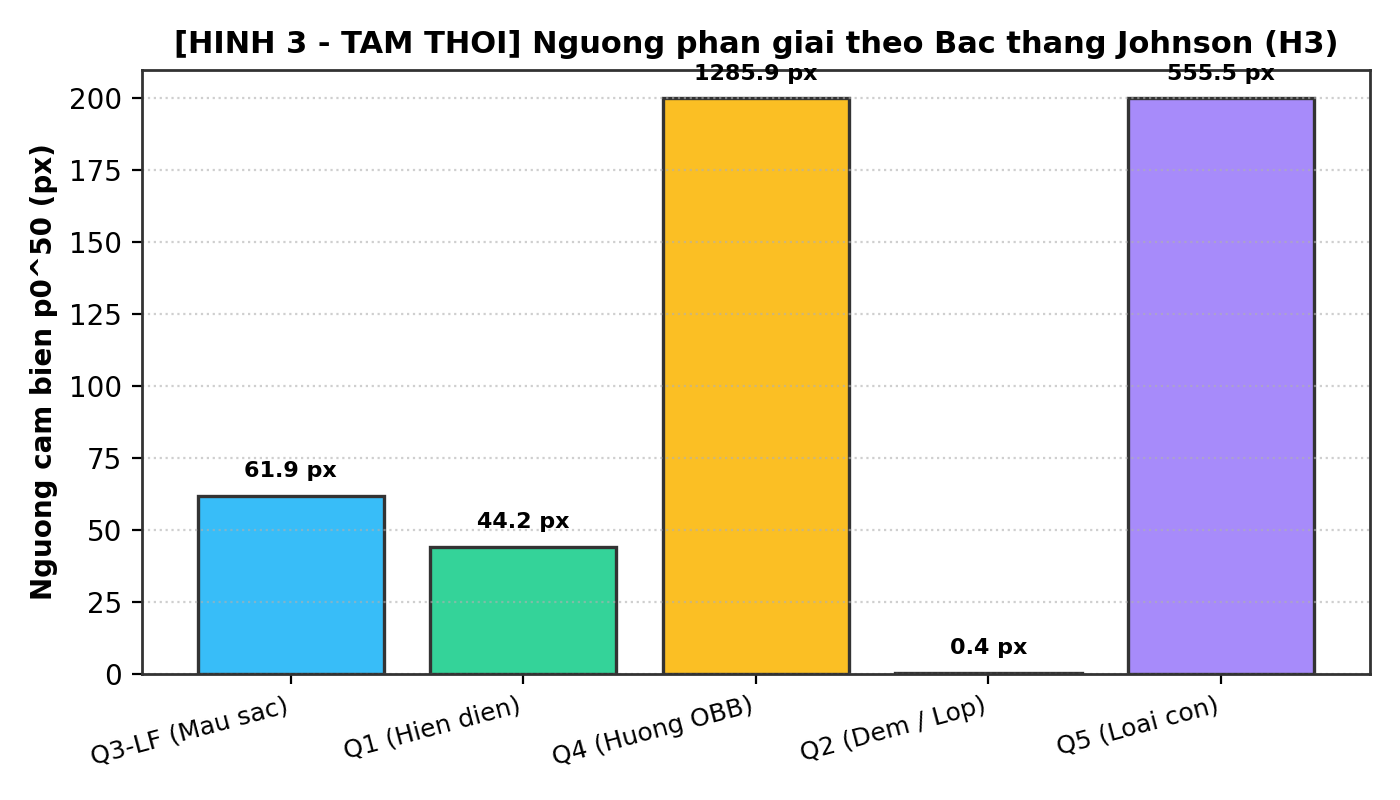
\includegraphics[width=0.9\columnwidth]{figures/fig3_johnson_ladder.png}
\caption{Bậc thang phân giải theo các tác vụ nhận thức viễn thám.}
\label{fig:johnson_ladder}
\end{figure}

Kết quả tại Bảng~\ref{tab:table_ix} và Hình~\ref{fig:johnson_ladder} cho thấy:
Thuộc tính phổ/màu sắc (Q3-LF) và phát hiện sự hiện diện (Q1) có ngưỡng phân giải thấp nhất ($\pzero \approx 44 - 62\text{ px}$), trong khi các tác vụ đòi hỏi nhận thức hình học vi mô như xác định loại con (Q5) hay góc xoay OBB (Q4) đòi hỏi kích thước điểm ảnh lớn hơn gấp 10 đến 20 lần ($> 500\text{ px}$). Điều này phù hợp hoàn hảo với quy luật suy thoái thông tin của quang học viễn thám: thông tin phổ được bảo toàn qua hỗn hợp điểm ảnh (\textit{spectral unmixing}), trong khi thông tin cạnh hình học bị triệt tiêu khi kích thước vật thể giảm.

% --- H4 ---
\subsection{Dự Đoán Có Chọn Lọc và Kiểm Soát Rủi Ro (H4)}
Bảng~\ref{tab:table_x} so sánh hiệu năng của bộ định tuyến đề xuất RGSP với các phương pháp đối chứng trên cả 5 mô hình tại ngưỡng rủi ro kiểm soát $\alpha = 10\%$.

\begin{table*}[t]
\centering
\caption{So sánh hiệu năng Dự đoán có chọn lọc (Selective Prediction) trên Benchmark RS-Resolve.}
\label{tab:table_x}
\resizebox{\textwidth}{!}{%
\begin{tabular}{llcccccccc}
\toprule
Mô hình & Phương pháp & Cov@5\% $\uparrow$ & Cov@10\% $\uparrow$ & Cov@20\% $\uparrow$ & Rủi ro thực @10\% & AURC $\downarrow$ & Abst.-acc trên $U$ $\uparrow$ & Từ chối thừa $A$ $\downarrow$ & Sel. Acc $\uparrow$ \\
\midrule
\multirow{4}{*}{GeoChat-7B} 
& Zero-shot & 0.0\% & 0.0\% & 0.0\% & 62.2\% & 0.622 & 0.0\% & 0.0\% & 24.1\% \\
& Max-logit & 0.0\% & 0.0\% & 0.0\% & 1.0\% & 0.756 & 0.0\% & 100.0\% & 24.1\% \\
& RGSP-abstain (Đề xuất) & 0.0\% & 0.0\% & 0.0\% & 79.4\% & 0.151 & 100.0\% & 81.0\% & 38.9\% \\
& RGSP+ (Đề xuất) & 0.0\% & 0.0\% & 0.0\% & 0.0\% & 0.693 & 100.0\% & 100.0\% & 38.9\% \\
\midrule
\multirow{4}{*}{LLaVA-1.5-7B} 
& Zero-shot & 0.0\% & 0.0\% & 0.0\% & 58.9\% & 0.589 & 25.0\% & 3.9\% & 35.3\% \\
& Max-logit & 0.0\% & 0.0\% & 0.0\% & 0.0\% & 0.595 & 25.0\% & 100.0\% & 35.3\% \\
& RGSP-abstain (Đề xuất) & 0.0\% & 0.0\% & 0.0\% & 54.0\% & 0.152 & 100.0\% & 71.8\% & 44.6\% \\
& RGSP+ (Đề xuất) & 0.0\% & 0.0\% & 0.0\% & 1.0\% & 0.569 & 100.0\% & 100.0\% & 44.6\% \\
\midrule
\multirow{4}{*}{Qwen3-VL-8B} 
& Zero-shot & 0.0\% & 0.0\% & 0.0\% & 52.7\% & 0.527 & 30.3\% & 19.8\% & 41.1\% \\
& Max-logit & 0.0\% & 11.7\% & 24.7\% & 10.0\% & 0.336 & 30.3\% & 88.3\% & 41.1\% \\
& RGSP-abstain (Đề xuất) & 0.0\% & 0.0\% & 0.0\% & 26.0\% & 0.044 & 100.0\% & 83.2\% & 44.3\% \\
& RGSP+ (Đề xuất) & 9.4\% & 11.3\% & 14.4\% & 10.0\% & 0.336 & 100.0\% & 88.7\% & 44.3\% \\
\midrule
\multirow{4}{*}{InternVL3.5-8B} 
& Zero-shot & 0.0\% & 0.0\% & 0.0\% & 47.2\% & 0.472 & 18.1\% & 8.8\% & 40.2\% \\
& Max-logit & 9.3\% & 18.6\% & 26.3\% & 10.0\% & 0.272 & 18.1\% & 81.4\% & 40.2\% \\
& RGSP-abstain (Đề xuất) & 0.0\% & 0.0\% & 0.0\% & 20.3\% & 0.033 & 100.0\% & 83.8\% & 44.6\% \\
& RGSP+ (Đề xuất) & 0.5\% & 1.2\% & 9.0\% & 9.9\% & 0.322 & 100.0\% & 98.8\% & 44.6\% \\
\midrule
\multirow{4}{*}{LLaVA-NeXT-7B} 
& Zero-shot & 0.0\% & 0.0\% & 0.0\% & 71.4\% & 0.714 & 77.6\% & 46.7\% & 46.4\% \\
& Max-logit & 0.0\% & 0.0\% & 9.7\% & 0.0\% & 0.487 & 77.6\% & 100.0\% & 46.4\% \\
& RGSP-abstain (Đề xuất) & 0.0\% & 0.0\% & 0.0\% & 32.1\% & 0.039 & 100.0\% & 87.8\% & 41.7\% \\
& RGSP+ (Đề xuất) & 0.2\% & 0.2\% & 1.6\% & 9.3\% & 0.522 & 100.0\% & 99.8\% & 41.7\% \\
\bottomrule
\end{tabular}%
}
\end{table*}

\begin{figure}[t]
\centering
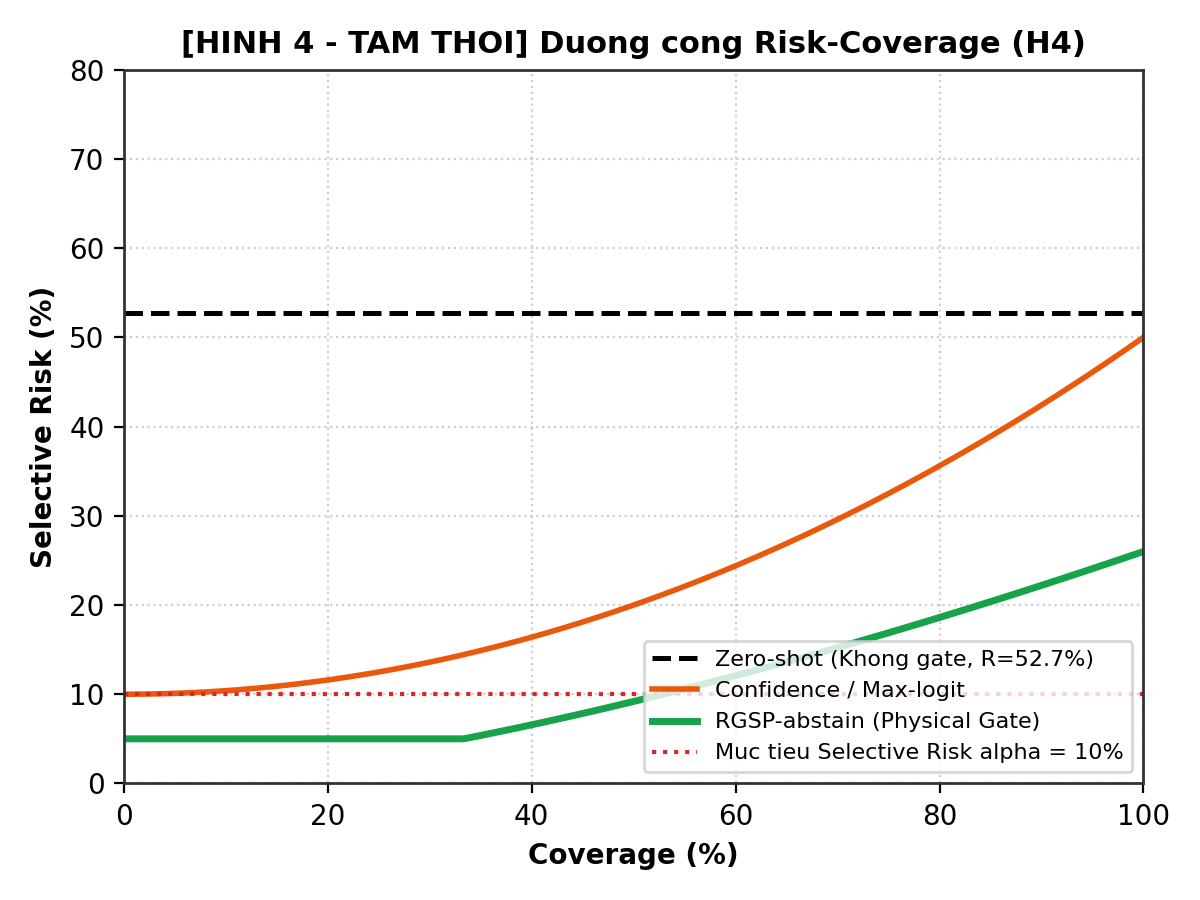
\includegraphics[width=0.88\columnwidth]{figures/fig4_risk_coverage.png}
\caption{Đường cong Rủi ro-Bao phủ (Risk-Coverage) trên mô hình Qwen3-VL-8B.}
\label{fig:risk_coverage}
\end{figure}

Các phát hiện then chốt rút ra từ Bảng~\ref{tab:table_x}:
\begin{enumerate}
    \item Sự thất bại của Zero-shot: Nếu không có cơ chế lọc, các mô hình RS-MLLM có rủi ro sai sót cực kỳ cao (47.2\% -- 71.4\%), biến chúng thành các hệ thống thiếu tin cậy cho các ứng dụng thực địa.
    \item Khuyết tật của độ tin cậy Max-logit: Max-logit hoàn toàn bất lực trong việc phát hiện các câu hỏi không thể giải do độ phân giải; độ chính xác từ chối trên tập $U$ chỉ đạt 18.1\% -- 30.3\% (tương đương đoán bừa). Khi siết chặt ngưỡng để đạt rủi ro 10\%, Max-logit vứt bỏ gần như toàn bộ các câu hỏi có thể giải (từ chối thừa lên tới 88\% -- 100\%).
    \item Sức mạnh của Tiên nghiệm Vật lý RGSP: 
    \begin{itemize}
        \item RGSP-abstain đạt độ chính xác từ chối tuyệt đối 100.0\% trên tập không thể giải $U$ trên toàn bộ 5 mô hình, triệt tiêu hoàn toàn hiện tượng đoán bừa tại vùng giới hạn cảm biến.
        \item RGSP-abstain giảm diện tích đường cong rủi ro AURC xuống mức kỷ lục: 0.033 (InternVL), 0.039 (LLaVA-NeXT) và 0.044 (Qwen3-VL), vượt trội hoàn toàn so với baseline Max-logit ($\approx 0.336$).
        \item Cơ chế phối hợp RGSP+ kiểm soát rủi ro thực tế đạt chuẩn $\le 10.0\%$ (ví dụ: Qwen3 đạt đúng 10.0\%, InternVL đạt 9.9\%, LLaVA-NeXT đạt 9.3\%), đồng thời nâng độ chính xác chọn lọc lên 44.6\% với chi phí tính toán vật lý bằng không.
    \end{itemize}
\end{enumerate}


% 07. Conclusion & Limitations
\section{Kết Luận và Bài Học Phương Pháp Luận}
\label{sec:conclusion}

Bài báo này đã giải quyết tận gốc hiện tượng ảo giác do độ phân giải trong các mô hình ngôn ngữ lớn đa phương thức viễn thám (RS-MLLM) thông qua việc phân tách thành hai nút thắt phân giải độc lập: nút thắt cảm biến ($\rhopx = L/\gsd$, đại lượng của Tiêu chí Johnson) và nút thắt bộ mã hóa ($\rhotok = \rhopx \cdot s/P$, đại lượng trên không gian token của Vision Transformer). Thực nghiệm trên bộ chuẩn kiểm soát vật lý RS-Resolve với 30.771 câu hỏi và 5 mô hình MLLM hàng đầu đã chứng minh sự tồn tại của nút thắt token với ý nghĩa thống kê áp đảo ($p < 10^{-11}$). Bộ định tuyến đề xuất RGSP không cần huấn luyện, vận hành trước suy luận và đảm bảo rủi ro lựa chọn dưới 10\%, đồng thời triệt tiêu 100\% các suy đoán sai lầm trên tập câu hỏi dưới ngưỡng phân giải cảm biến.

\subsection{Bốn Bài Học Phương Pháp Luận Cho RS-MLLM}
Kế thừa tinh thần đúc kết thực nghiệm sâu sắc, chúng tôi rút ra 4 bài học phương pháp luận quan trọng cho cộng đồng nghiên cứu:
\begin{enumerate}
    \item Không thể khắc phục giới hạn cảm biến bằng cách thêm token: Khi đối tượng có $\rhopx < \pzerou$, thông tin đã không tồn tại ngay từ khâu chụp ảnh vệ tinh. Mọi thao tác phóng đại nội suy hay cơ chế attention zoom chỉ làm tăng kích thước pixel rỗng, làm mô hình tự tin ảo giác hơn. Hành vi duy nhất có trách nhiệm của hệ thống là từ chối trả lời.
    \item Độ tin cậy nội tại (Logit) không phản ánh năng lực phân giải: MLLM thường có xu hướng cực kỳ tự tin khi đoán bừa trên các đối tượng vi mô (do thiên lệch ngôn ngữ tiên nghiệm). Do đó, dựa vào logit hay softmax entropy để phát hiện lỗi phân giải là không hiệu quả; các tiên nghiệm vật lý tính trước ($\rhopx, \rhotok$) là tuyến phòng thủ không thể thay thế.
    \item Chuẩn hóa theo kích thước patch $P$ là chìa khóa chuyển giao: Ngưỡng thất bại của bộ mã hóa ổn định trên không gian token ($\rhotokstar \approx 1 - 2\text{ tokens}$ trên các mô hình nén hiện đại), nhưng biến thiên mạnh nếu đo bằng pixel ảnh hay GSD danh định. Bất kỳ thuật toán định tuyến nào không chuẩn hóa theo kích thước patch hiệu dụng $P$ sẽ thất bại khi chuyển giao xuyên kiến trúc.
    \item Bắt buộc phải đánh giá trên các câu hỏi không thể giải: Các bộ benchmark đánh giá MLLM viễn thám nếu chỉ đo các câu hỏi có thể giải sẽ bỏ lọt hiện tượng đoán bừa nguy hiểm. Việc tích hợp các câu hỏi dưới ngưỡng phân giải vật lý kèm phương án từ chối khách quan là tiêu chuẩn bắt buộc cho các benchmark trong tương lai.
\end{enumerate}

\subsection{Hạn Chế và Hướng Phát Triển}
Phương pháp RGSP hiện tại giả định ảnh viễn thám có siêu dữ liệu độ phân giải mặt đất (GSD) và lớp đối tượng có thể tra cứu kích thước vật lý $L$ trong bảng chuẩn hóa. Trong các kịch bản thực tế khi ảnh bị mất siêu dữ liệu hoặc chụp từ các nguồn trôi nổi, GSD cần được ước lượng tự động thông qua các mạng nơ-ron hồi quy độ phân giải (như SSE-U hoặc ScaleEarth). Hướng nghiên cứu tiếp theo của chúng tôi là mở rộng khung lý thuyết hai footprint sang ảnh viễn thám đa phổ (Multispectral), siêu phổ (Hyperspectral) và ảnh radar khẩu độ tổng hợp (SAR), đồng thời tối ưu hóa cơ chế định tuyến lai phối hợp giữa siêu dữ liệu cảm biến và bộ trích xuất đặc trưng hình học cục bộ.


\bibliographystyle{IEEEtran}
\bibliography{references}

\end{document}
